\documentclass[a4paper,10pt]{exam}

\usepackage[utf8]{inputenc}
\usepackage[cyr]{aeguill}
\usepackage[francais]{babel}
\usepackage{fullpage}
\usepackage{amsmath}
\usepackage{array}
\usepackage{tikz}
\input kvmacros
\usetikzlibrary{arrows,shapes,trees,patterns,fit,backgrounds,%
decorations.pathreplacing,chains,calc,decorations.pathmorphing,matrix,circuits.logic.CDH,automata}

\ifthenelse{\equal{\detokenize{correction}}{\jobname}}
{\printanswers}
{\noprintanswers}

\title{Architecture des ordinateurs - TD 09}

\author{}
\date{}

\begin{document}
\maketitle


\section{Machine à états}

Soit l'automate suivant. Les états du graphe sont les états (représentés sur
deux bits $S = s_1s_2$), les arcs sont les transitions commandées par deux
signaux binaires $A$ et $B$.

\begin{center}
\begin{tikzpicture}[shorten >=1pt,node distance=2cm,on grid,auto]
\node[state,initial] (q_0) {$00$};
\node[state] (q_1) [above right=of q_0] {$01$};
\node[state] (q_2) [below right=of q_0] {$10$};
\node[state,accepting](q_3) [below right=of q_1] {$11$};
\path[->] (q_0) edge              node        {$A$} (q_1)
                edge              node [swap] {$\overline{A}$} (q_2)
          (q_1) edge              node        {$A$} (q_3)
                edge [loop above] node        {$B.\overline{A}$} ()
          (q_2) edge              node [swap] {$\overline{B}$} (q_3)
                edge [loop above] node        {$B$} ()
          (q_3) edge [loop above] node        {$1$} ();
\end{tikzpicture}
\end{center}

On souhaite réaliser cet automate en logique synchrone. À chaque front
d'horloge, l'automate peut changer d'état en fonction des valeurs de $A$ et
de $B$.

Il existe une manière systématique de réaliser des machines à état en logique
synchrone:

\begin{center}
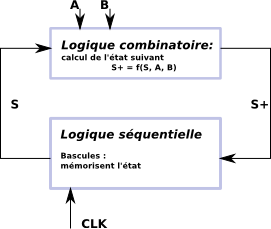
\includegraphics{TD9-automate}
\end{center}
\begin{enumerate}
  \item Pour l'automate ci-dessus, donner la fonction $S+ = f(S, A, B)$ (table de
    vérité ou expression booléenne).
    \begin{solution}

      On choisit de représenter la fonction f avec une table de vérité:

      \begin{verbatim}
      S  | A B | S+
      ---+-----+---
      00 | 0 X | 10
         | 1 X | 01
      ---+-----+---
      01 | 1 X | 11
         | 0 1 | 01
         | 0 0 | XX
      ---+-----+---
      10 | X 1 | 10
         | X 0 | 11
      ---+-----+---
      11 | X X | 11
      \end{verbatim}
    \end{solution}
  \item Simplifier la fonction $f$.
    \begin{solution}
      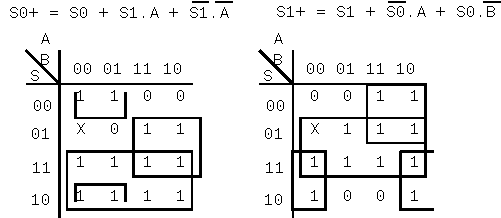
\includegraphics{TD9-auto}
    \end{solution}
  \item Proposer un circuit pour la partie combinatoire du schéma.
    \begin{solution}
      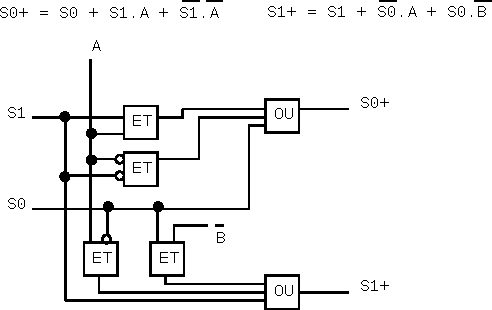
\includegraphics{TD9-auto1}
    \end{solution}

  \item Proposer un circuit pour la partie séquentielle du schéma (en utilisant
    des bascules D).
    \begin{solution}
      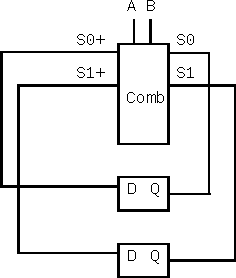
\includegraphics{TD9-auto2}
    \end{solution}

\end{enumerate}

\section{Compteur de Parité}
Nous souhaitons calculer la parité de la somme des bits d'un mot binaire de
taille arbitraire reçu sur un port série. À chaque front de l'horloge on peut
lire sur l'entrée $D$ le bit suivant. Le signal $I$ est à zéro tout le temps
sauf pour le top d'horloge précédant le début d'un mot. Une bascule $D$ sera
utilisée pour calculer la parité du bit en cours.

\begin{enumerate}
  \item On souhaite réaliser le circuit ci-dessus en utilisant une seule bascule
    D. Quelle est l'équation de $Q^{+} = f(Q,D,I)$ sachant que $Q^{+}$ est la
    parité de tous les bits reçus depuis le dernier top de $I$.

    \begin{solution}
      $$Q^+ = (D \oplus Q).I $$
    \end{solution}
  \item Donner le schéma du circuit.
    \begin{solution}
      Avec une bascule D il suffit de prendre l'équation ci-dessus.
      Avec une bascule T il suffit d'implémenter le reset du signal I en
      utilisant par exemple un multiplexeur sur l'entrée T qui choisit entre
      D et $\overline{Q}$ en fonction de I.
    \end{solution}
\end{enumerate}

\section{Distributeur de café}
Nous souhaitons réaliser le contrôleur d'un distributeur de café.
Ce dernier accepte uniquement des pièces de 5 et 10 centimes.
Le prix d'un café est de 15 centimes.

Il faut faire l'appoint:
\begin{itemize}
  \item Si la somme des pièces introduites dépasse 15 centimes, toutes les
    pièces sont rendues.
  \item Si la somme des pièces introduites fait 15 centimes exactement, la
    boisson est distribuée.
\end{itemize}

Remarques:
\begin{itemize}
  \item La période d'horloge est négligeable devant le temps d'introduction
    d'une pièce. On fait l'hypothèse qu'au moins un cycle d'horloge s'écoule
    entre l'introduction de deux pièces.
  \item Un signal entrant $I$ sur deux bits signale l'introduction de pièces :
    00 $\rightarrow$ aucune pièce introduite, 01 $\rightarrow$ pièce de 5
    centimes, 10 $\rightarrow$ pièce de 10 centimes.
  \item Le signal sortant $D$ commande la  distribution d'un café.
  \item Le signal sortant $R$ commande le rendu des pièces.
\end{itemize}

\begin{enumerate}
  \item Représentez l'automate modélisant le comportement du distributeur.
  \item Combien de bits faut-il pour coder l'état de la machine ? Numérotez
    les états dans l'ordre naturel croissant (0,1,$\dots$).

    \begin{solution}
      Il y a 5 états, il faut donc 3 bits.

      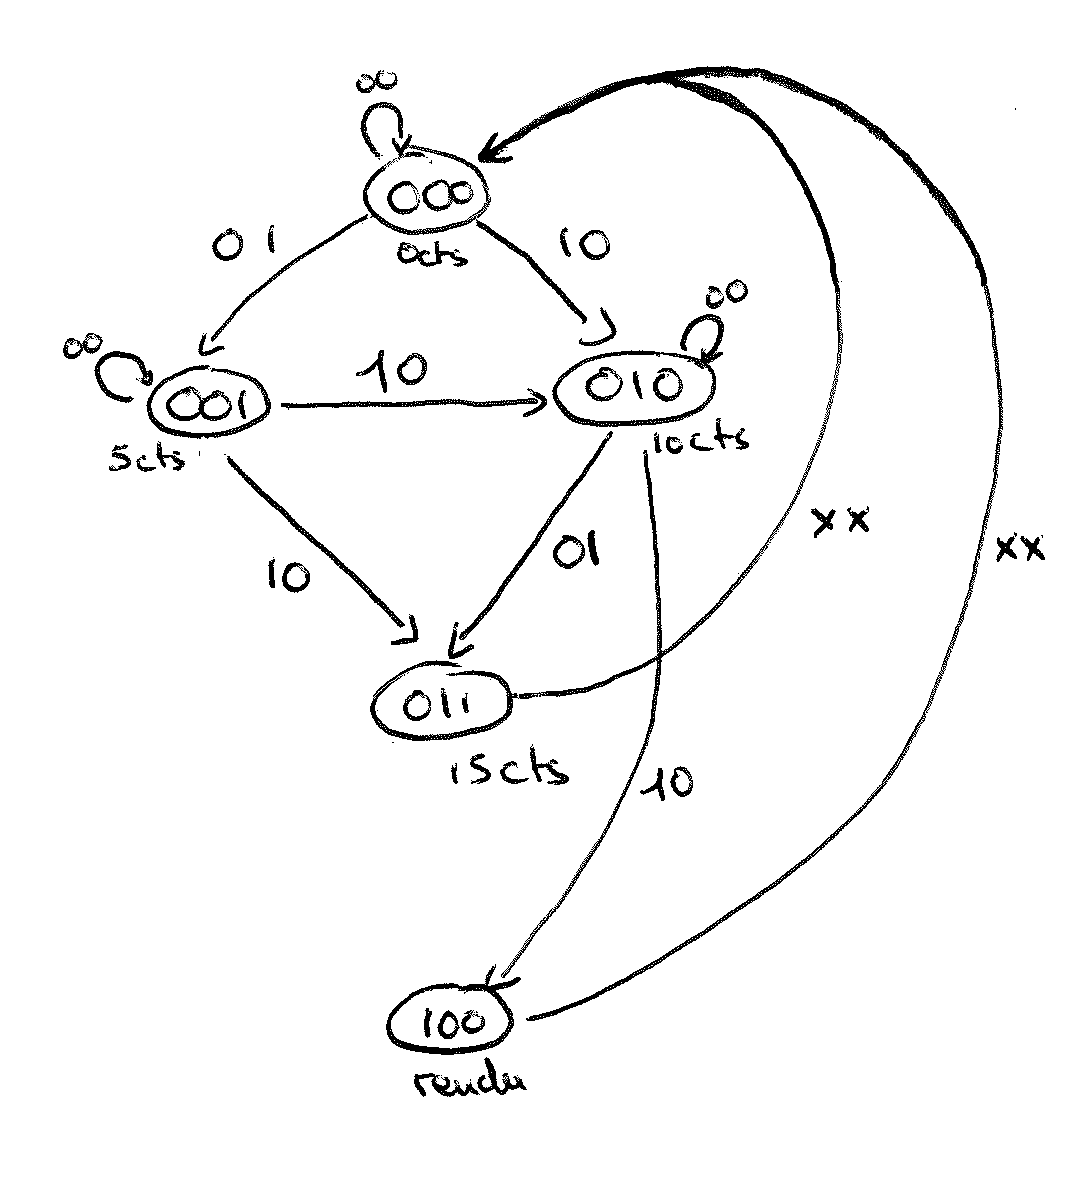
\includegraphics{TD9-transitions}
    \end{solution}

  \item Dressez la table de vérité reliant l'état précédent $Q$,
    l'entrée $I$,  l'état suivant $Q^{+}$ et $D$ et $R$.

    \begin{solution}
\begin{verbatim}
   10   210   210
   I  | Q   | Q+  | D R
   ---+-----+-----+----
   00 | 000 | 000 |
      | 001 | 001 |
      | 010 | 010 |
      | 011 | 000 |
      | 100 | 000 |
   ---+-----+-----+----
   01 | 000 | 001 |
      | 001 | 010 |
      | 010 | 011 | 1
      | 011 | 000 |
      | 100 | 000 |
   ---+-----+-----+----
   10 | 000 | 010 |
      | 001 | 011 | 1
      | 010 | 100 |  1
      | 011 | 000 |
      | 100 | 000 |
   ---+-----+-----+----
   11 | XXX | XXX |
   XX |>100 | XXX |
\end{verbatim}

    \end{solution}
  \item Pouvez vous trouver directement une expression minimale pour $Q_2^{+}$
    en fonction de $Q$ et $I$.
      \begin{solution}
        Il y a un seul minterm pour lequel $Q_2^{+}$ est vrai (10010). En le
        combinant avec les don't care on peut le simplifier:
        $$Q_2^{+} = m(10010) + d(XX1X1, XXX11X, 11XXX) = I_1.Q_1.\overline{Q_0}$$
      \end{solution}

  \item En utilisant la méthode de Quine McCluskey trouvez des expressions
    minimales pour $Q_1^{+}$ et $Q_0^{+}$ en fonction de $Q$ et $I$.
    \begin{solution}
      $$Q_0^{+} = \sum m(1,8,10,17) + d(5,6,7,13,14,15,21,\dots,31)$$
      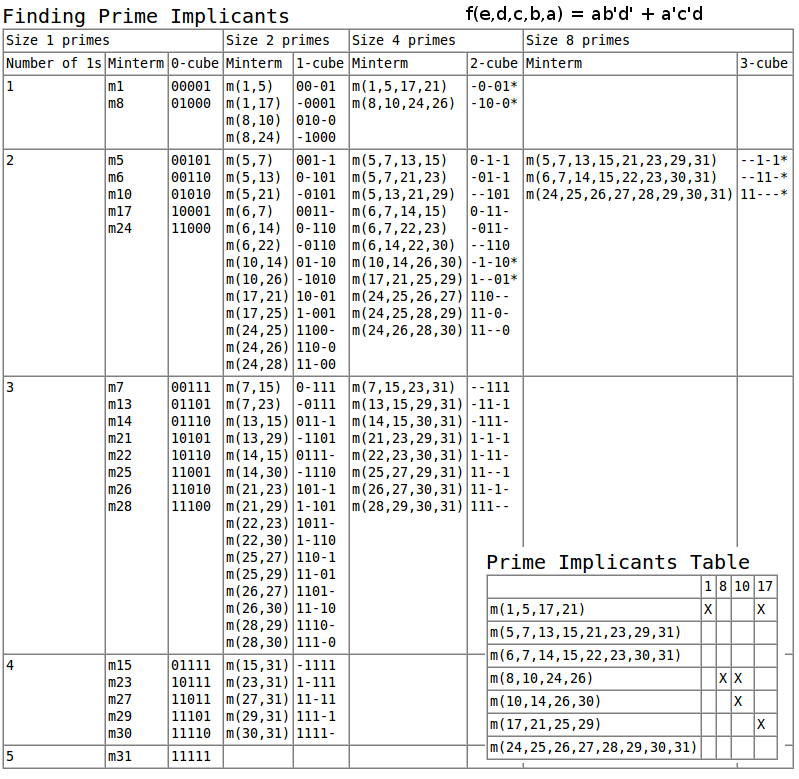
\includegraphics[width=.8\textwidth]{10MC2}
      $$Q_0^{+} = Q_0.\overline{Q_1}.\overline{I_0} +
      \overline{Q_0}.\overline{Q_2}.I_0$$

      $$Q_1^{+} = \sum m(2,9,10,16,17) + d(5,6,7,13,14,15,21,\dots,31)$$
      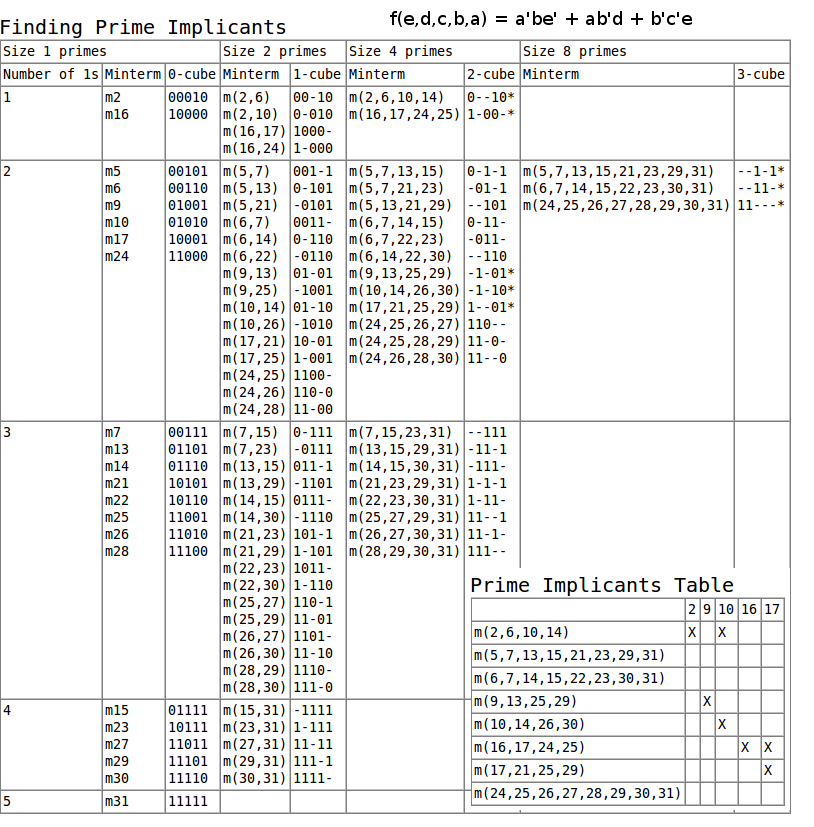
\includegraphics[width=.8\textwidth]{10MC1}
      $$Q_1^{+} = \overline{Q_0}.Q_1.\overline{I_1} +
      Q_0.\overline{Q_1}.I_0 + \overline{Q_1}.\overline{Q_2}.I_1$$
    \end{solution}

  \item Exprimez $D$ et $R$ en fonction de $Q^{+}$.
    \begin{solution}
      $R$ est vrai uniquement lorsque $Q^+_2$ est vrai: $R = Q^+_2$

      $D$ est vrai uniquement lorsque $Q^+_1$ et $Q^+_0$ sont vrais: $D = Q^+_0.Q^+_1$
    \end{solution}
  \item Réalisez un circuit pour le contrôleur.
    \begin{solution}
      Même technique que pour l'exercice 1. Vous disposez de toutes les
      équations pour réaliser la partie combinatoire du circuit. Il suffit de
      rajouter autant de bascules D que d'états et les utiliser pour faire une
      boucle entre $Q^+$ et $Q$.
    \end{solution}
\end{enumerate}


\end{document}
